\begin{figure*}[!htbp]
	\centering
	\IfFileExists{sec/figs/25 - Generation Result.png}%
	{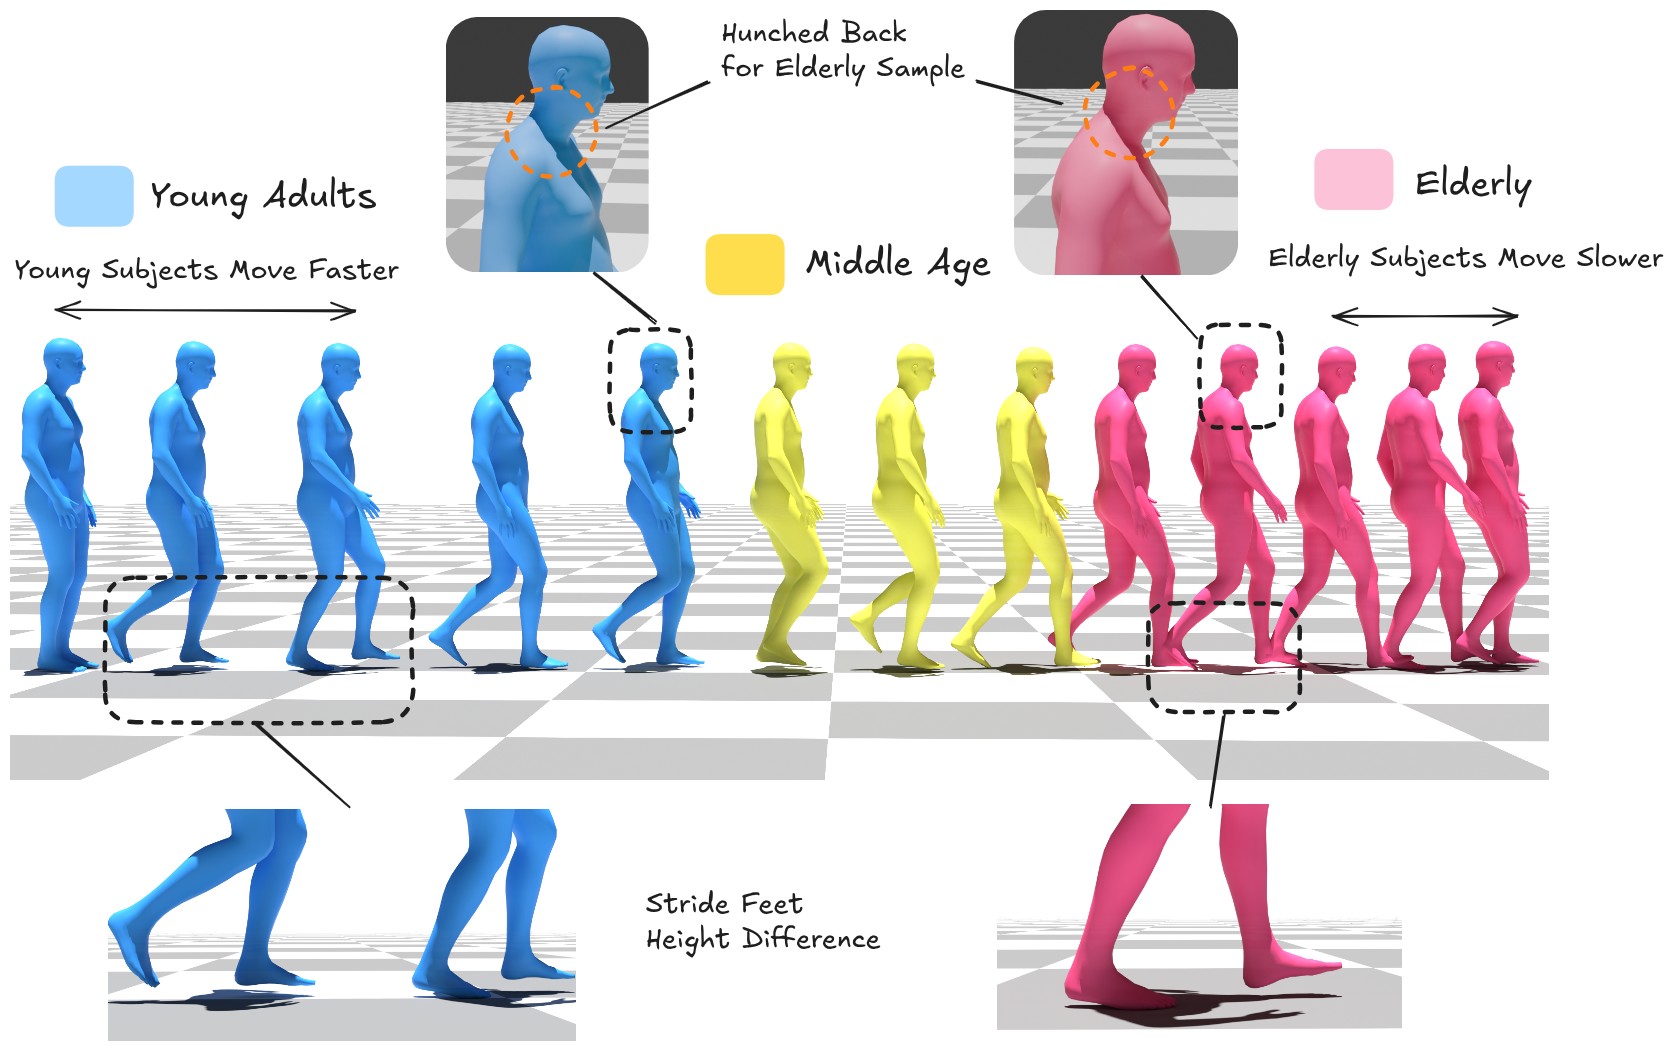
\includegraphics[width=0.75\textwidth]{sec/figs/25 - Generation Result.png}}%
	{\fbox{\parbox[c][2cm][c]{0.75\textwidth}{\centering Figure missing: \texttt{sec/figs/25 - Generation Result.png}}}}
	\caption{Generated walking sequences across the three age tokens (Young, Mid-age, Elderly).}
	\label{fig:qualitative}
\end{figure*}

\subsection{Data Quality}
\label{sec:exp-data}

When processing the Van Criekinge et al.~\cite{vancriekinge2023dataset} clinical motion capture dataset, we must ensure that biological fidelity is preserved during the conversion to the HumanML3D feature representation. We adapt the prior-space optimization method from VPoser~\cite{pavlakos2019expressivebodycapture3d} --- which fits SMPL parameters in a learned VAE latent pose space to bias solutions toward plausible human poses --- and design a multi-stage fitting pipeline with the loss weights in Table~\ref{tab:smpl_fit}.
The first stage recovers the global body pose and the second stage refines body shape against the pose prior.
Fig.~\ref{fig:optplots} shows the rapid convergence of the fitting loss, yielding successful recovery of the body parameters and effective elimination of the mesh inflation and crouch-walking artifacts (Fig.~\ref{fig:artifact}).

\begin{table}[H]
    \centering
    \caption{Two-stage SMPL fitting configuration. The L-BFGS optimizer runs in VPoser latent pose space with \texttt{max\_iter}=400, \texttt{lr}=1.0, \texttt{tolerance\_change}=$10^{-4}$, history size 200. $\lambda_\text{data}$ matches markers to SMPL surface vertices; $\lambda_{\boldsymbol{\beta}}$ regularizes body shape toward zero; $\lambda_\text{poZ}$ regularizes the VPoser latent pose.}
    \label{tab:smpl_fit}
    \begin{tabular}{lccc}
        \toprule
        \textbf{Stage} & $\lambda_\text{data}$ & $\lambda_{\boldsymbol{\beta}}$ & $\lambda_\text{poZ}$ \\
        \midrule
        1. Shape-free local minimum & 10.0 & 0.00 & 0.08 \\
        2. Shape \& prior refinement & 10.0 & 0.10 & 0.02 \\
        \bottomrule
    \end{tabular}
\end{table}

\begin{figure}[H]
	\centering
	\IfFileExists{sec/figs/loss_plt.png}%
	{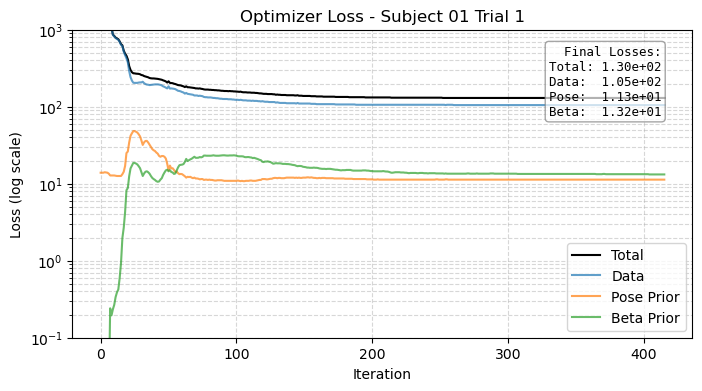
\includegraphics[width=0.7\linewidth]{sec/figs/loss_plt.png}}%
	{\fbox{\parbox[c][1.2cm][c]{\linewidth}{\centering Loss plot missing: \texttt{sec/figs/loss_plt.png}}}}
	\caption{Loss during multi-stage VPoser fitting for Subject 01.}
	\label{fig:optplots}
\end{figure}

The dataset was originally collected for the purpose of health statistics computation, with a relatively lower quality compared to modern SOTA data capture sets~\cite{mahmood2019amass}.
To make the data ready for deep learning use, we resolved dataset-specific artifacts during data processing, including sensor measurement errors, initialization transients, and mislabeled markers, through a multi-stage pipeline.
Our procedure is as follows: (1) we delete clips that are too short ($<40$ frames); (2) we rank the SMPL-fitted clips by their final marker-reconstruction loss; (3) we perform manual visual inspection at the high-loss tail to remove clips with missing markers, labeling errors, or other artifacts.
After this filtering and a $\pm 5$-frame boundary trim to remove sensor initialization and shutdown transients, the data loader yields 420 effective walking clips, stratified by chronological age as summarized in Table~\ref{tab:age_dist}.

\begin{table}[H]
    \centering
    \caption{Clip filtering and age distribution of the processed VC dataset (138 subjects).}
    \label{tab:age_dist}
    \begin{tabular}{lc}
        \toprule
        \textbf{Stage / Group} & \textbf{Clips} \\
        \midrule
        \multicolumn{2}{l}{\textit{Discarded}} \\
        \quad T-pose calibration clips (\texttt{\_0}) & 138 \\
        \quad Short clips ($<40$ frames) & 24 \\
        \quad Manual artifact removal & 4 \\
        \midrule
        \multicolumn{2}{l}{\textit{Effective (by age group)}} \\
        \quad Young (18--35) & 115 \\
        \quad Mid-age (35--60) & 154 \\
        \quad Elderly ($\geq 60$) & 151 \\
        \midrule
        \textbf{Total effective} & \textbf{420} \\
        \bottomrule
    \end{tabular}
\end{table}

\subsection{Age Classifier Training Results}
\label{sec:exp-classifier}

We fine-tuned the ST-GCN++ architecture as a three-class classifier under the age bins Young ($<35$), Mid-age (35--60), and Elderly ($\geq 60$).
To prevent subject-based overfitting --- where the model memorizes the individual gait patterns of specific subjects --- we ensured strict, mutually exclusive subject assignment between the training and validation splits.
The full training configuration is given in Table~\ref{tab:stgcn_config}.

\begin{table}[H]
    \centering
    \caption{ST-GCN++ age classifier training configuration.}
    \label{tab:stgcn_config}
    \begin{tabular}{ll}
        \toprule
        \textbf{Hyperparameter} & \textbf{Value} \\
        \midrule
        Backbone pretraining & NTU RGB+D 120 \\
        Unfrozen blocks & Block 8, Block 9 \\
        Trainable parameters & 718{,}713 (51.5\%) \\
        Loss & Class-weighted cross-entropy \\
        Class weights (Y / M / E) & 1.03 / 0.86 / 1.15 \\
        Optimizer & AdamW, weight decay $10^{-4}$ \\
        Learning rate & $10^{-3}$ (head), $10^{-4}$ (backbone) \\
        Schedule & Cosine annealing \\
        Batch size & 8 \\
        Train-time clip sampling & 1 random temporal clip / sample \\
        Val.\ aggregation & 10-clip prob.\ average \\
        \bottomrule
    \end{tabular}
\end{table}

\begin{figure}[H]
	\centering
	\begin{minipage}[t]{0.49\linewidth}
		\centering
		\IfFileExists{sec/figs/stgcn_train_loss.png}%
		{
\includegraphics[width=\linewidth]{sec/figs/stgcn_train_loss.png}}%
		{}
	\end{minipage}\hfill
	\begin{minipage}[t]{0.49\linewidth}
		\centering
		\IfFileExists{sec/figs/stgcn_val_accuracy.png}%
		{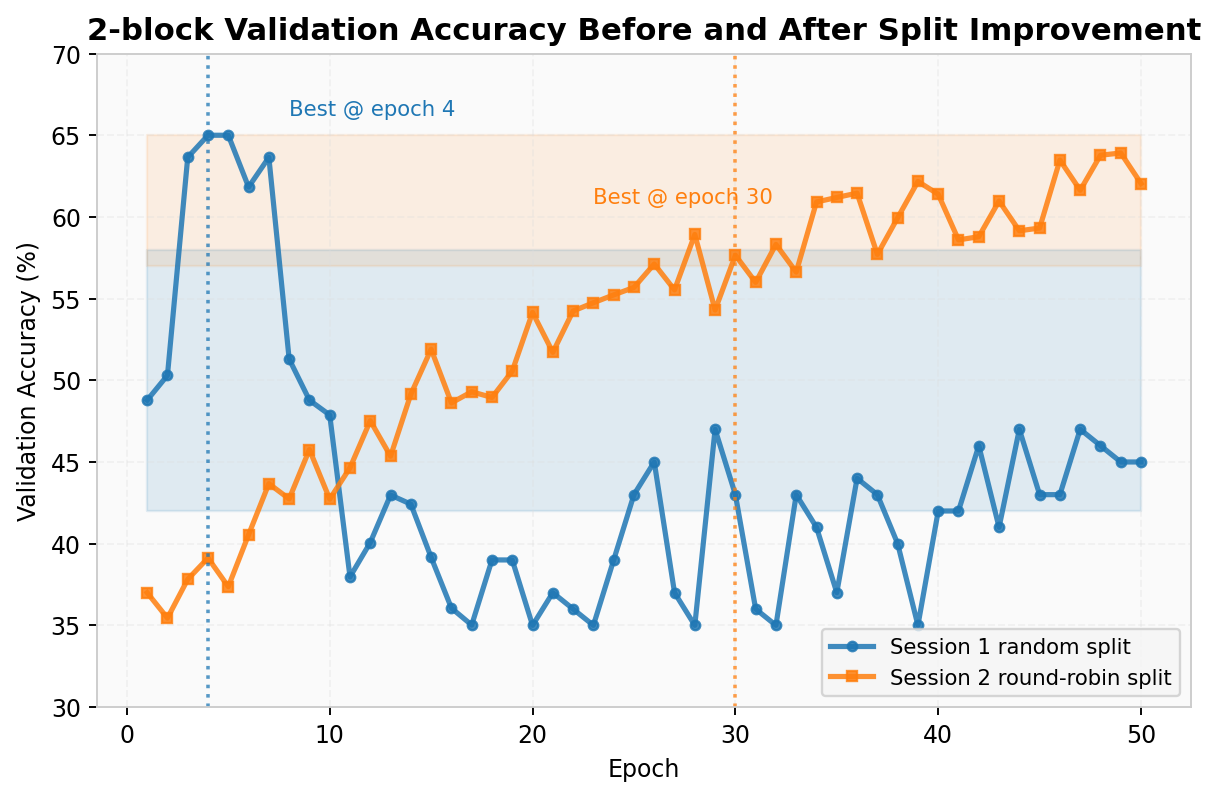
\includegraphics[width=\linewidth]{sec/figs/stgcn_val_accuracy.png}}%
		{}
	\end{minipage}
	\caption{Training dynamics for the ST-GCN age classifier. Left: training loss. Right: validation accuracy.}
	\label{fig:stgcn_curves}
\end{figure}

\begin{figure}[H]
	\centering
	\IfFileExists{sec/figs/stgcn_confusion.png}%
	{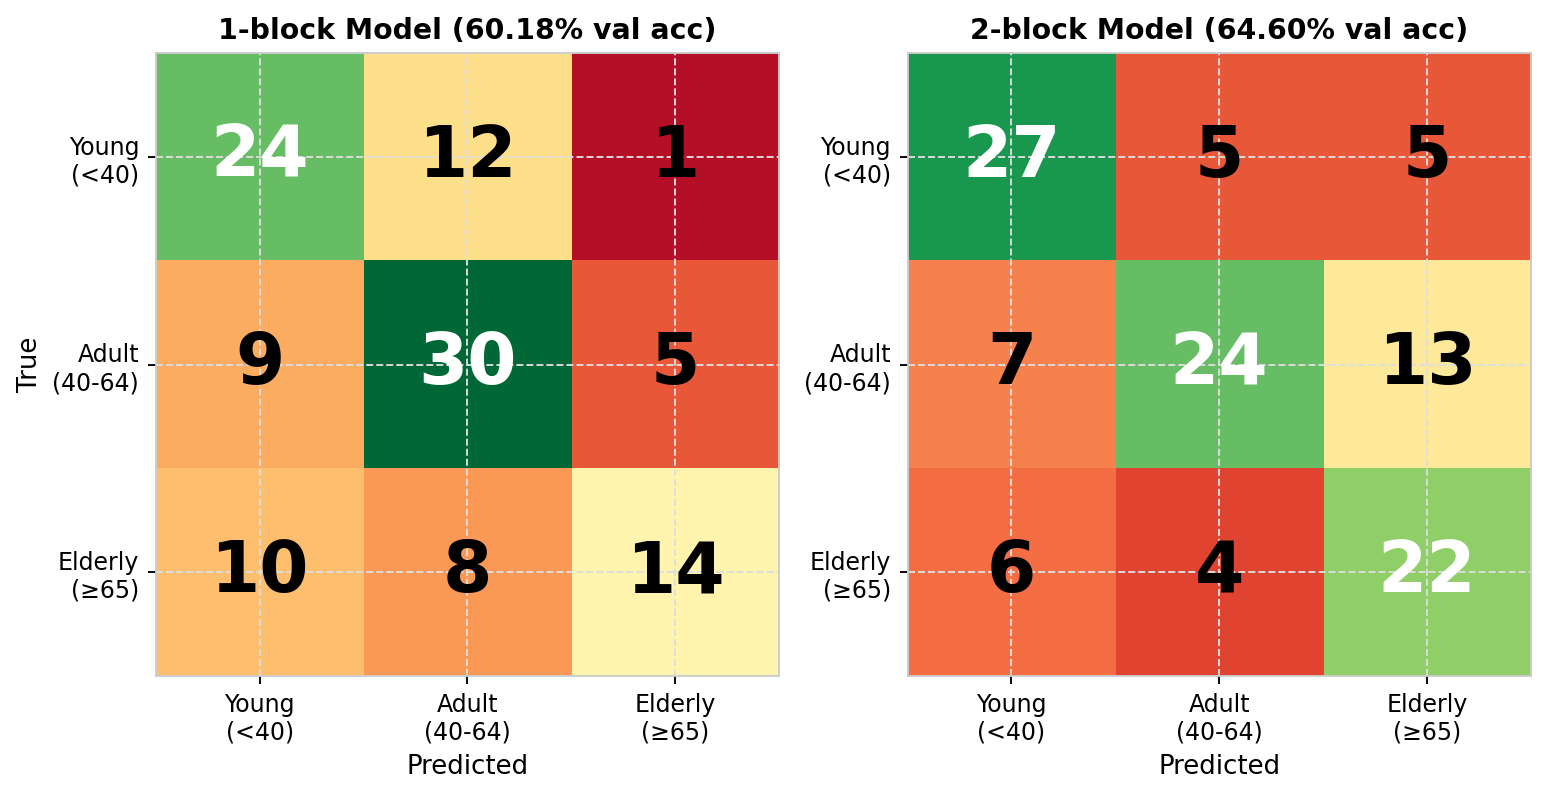
\includegraphics[width=0.8\linewidth]{sec/figs/stgcn_confusion.png}}%
	{}
	\caption{Confusion matrices for the ST-GCN predictions.}
	\label{fig:stgcn_confusion}
\end{figure}

As shown in the training dynamics (Fig.~\ref{fig:stgcn_curves}), we progressively unfreeze backbone blocks to balance validation accuracy (64.60\%) against overfitting.
Overfitting is still observed, as evidenced by the gap between validation accuracy and the near-perfect fit on the training split.
The confusion matrices (Fig.~\ref{fig:stgcn_confusion}) reveal that the model consistently segregates the kinematic extremes (Young vs.\ Elderly), with the primary failure mode being the fragmentation of the Mid-age category.
This indicates that, despite the dataset-size constraint, the classifier successfully encapsulates biomechanical signatures discriminating between age groups.
The Mid-age fragmentation is also a feature, not only a bug: clinical studies consistently find that the kinematic gap between Young and Mid-age groups is small relative to within-group variance~\cite{boyer2023nia, herssens2020investigation}, so the Mid-age condition is noisy as a trend anchor.
We therefore report quantitative gait-metric trends as Young$\to$Elderly contrasts and include the Mid-age condition primarily to give the classifier and adapter a smooth interior point rather than a hard binary boundary.

\subsection{Generative Motion Synthesis}
\label{sec:exp-gen}

We fine-tune the LoRA-adapted MDM under the configuration in Table~\ref{tab:lora_config}.
After training, we generate 9{,}000 motion clips (3{,}000 per age condition) from the walking prompt.
At inference we set the classifier-free guidance scale to $s = 1.0$ to match the conditional distribution learned during LoRA training and avoid extrapolation past the broader HumanML3D motion prior.

\begin{table}[H]
    \centering
    \caption{LoRA fine-tuning configuration.}
    \label{tab:lora_config}
    \begin{tabular}{ll}
        \toprule
        \textbf{Hyperparameter} & \textbf{Value} \\
        \midrule
        Base model & MDM, HumanML3D, 500k steps \\
        LoRA rank ($r$) & 12 \\
        Prior-preservation weight ($\lambda_\text{prior}$) & 1.0 \\
        Diffusion steps (training) & 1000 \\
        Training steps & 4000 \\
        Batch size & 32 \\
        Style tokens & \texttt{young}, \texttt{mid}, \texttt{old} \\
        Compute & 4$\times$V100 \\
        \bottomrule
    \end{tabular}
\end{table}

Fig.~\ref{fig:qualitative} shows representative motion sequences generated from the walking prompt under each age token.
Coarse, well-known stylistic cues of aging are visible: the Elderly sample exhibits a noticeably hunched back, and the stride-to-stride foot-clearance height differs visibly between the Young and Elderly conditions.
Visual inspection alone, however, is an unreliable proxy for the underlying biomechanics, motivating quantitative analysis.

\subsection{Quantitative Clinical Analysis}
\label{sec:exp-clinical}

We computed the standard clinical gait metrics (spatiotemporal parameters, gait variability, joint range of motion) on both the processed ground-truth dataset and the 9{,}000 generated motion clips.

\subsubsection{Dataset Baseline Validation}
Analysis of the ground-truth clinical data confirms that the expected aging signal is successfully preserved end-to-end through our conversion pipeline.
We observe monotonic Young$\to$Elderly trends consistent with clinical literature: walking speed decreases (1.22 to 1.10 m/s), stride length decreases (1.34 to 1.26 m), and knee RoM decreases ($54.9^\circ$ to $51.5^\circ$).
Conversely, stride-time CV increases from 8.9\% to 15.0\% (Fig.~\ref{fig:clinical_eval}).
Qualitatively, comparative heatmaps of joint angular velocity over a normalized gait cycle show that the elderly subject (Age 78) exhibits reduced peak velocities and constrained range of motion, whereas the young subject (Age 24) demonstrates distinct, high-intensity kinematic bursts (Fig.~\ref{fig:heatmap}).

\begin{figure}[H]
	\centering
	\IfFileExists{sec/figs/heatmap.png}%
	{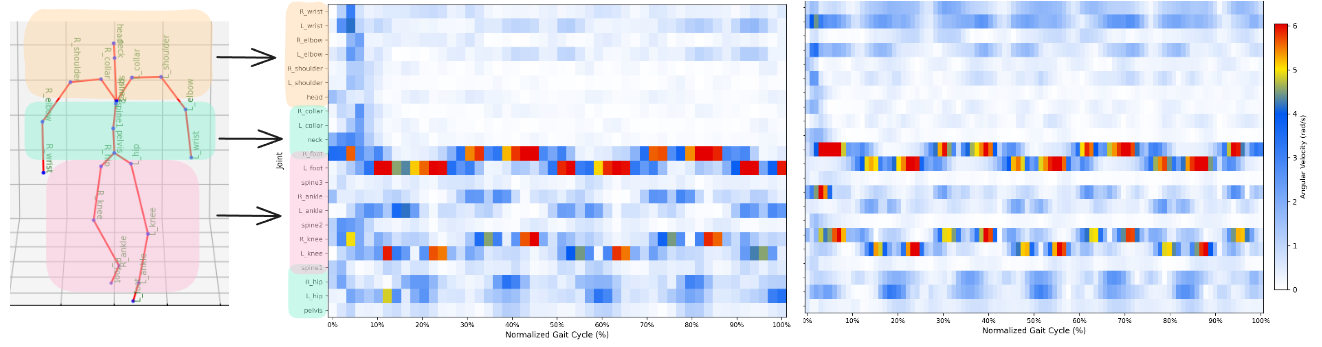
\includegraphics[width=\linewidth]{sec/figs/heatmap.png}}%
	{}
	\caption{Comparative heatmaps of joint angular velocity (rad/s) over a normalized gait cycle. Left: Young Subject (Age 24); Right: Elderly Subject (Age 78).}
	\label{fig:heatmap}
\end{figure}

\begin{figure}[H]
	\centering
	\IfFileExists{sec/figs/dataset/age_regression.png}%
	{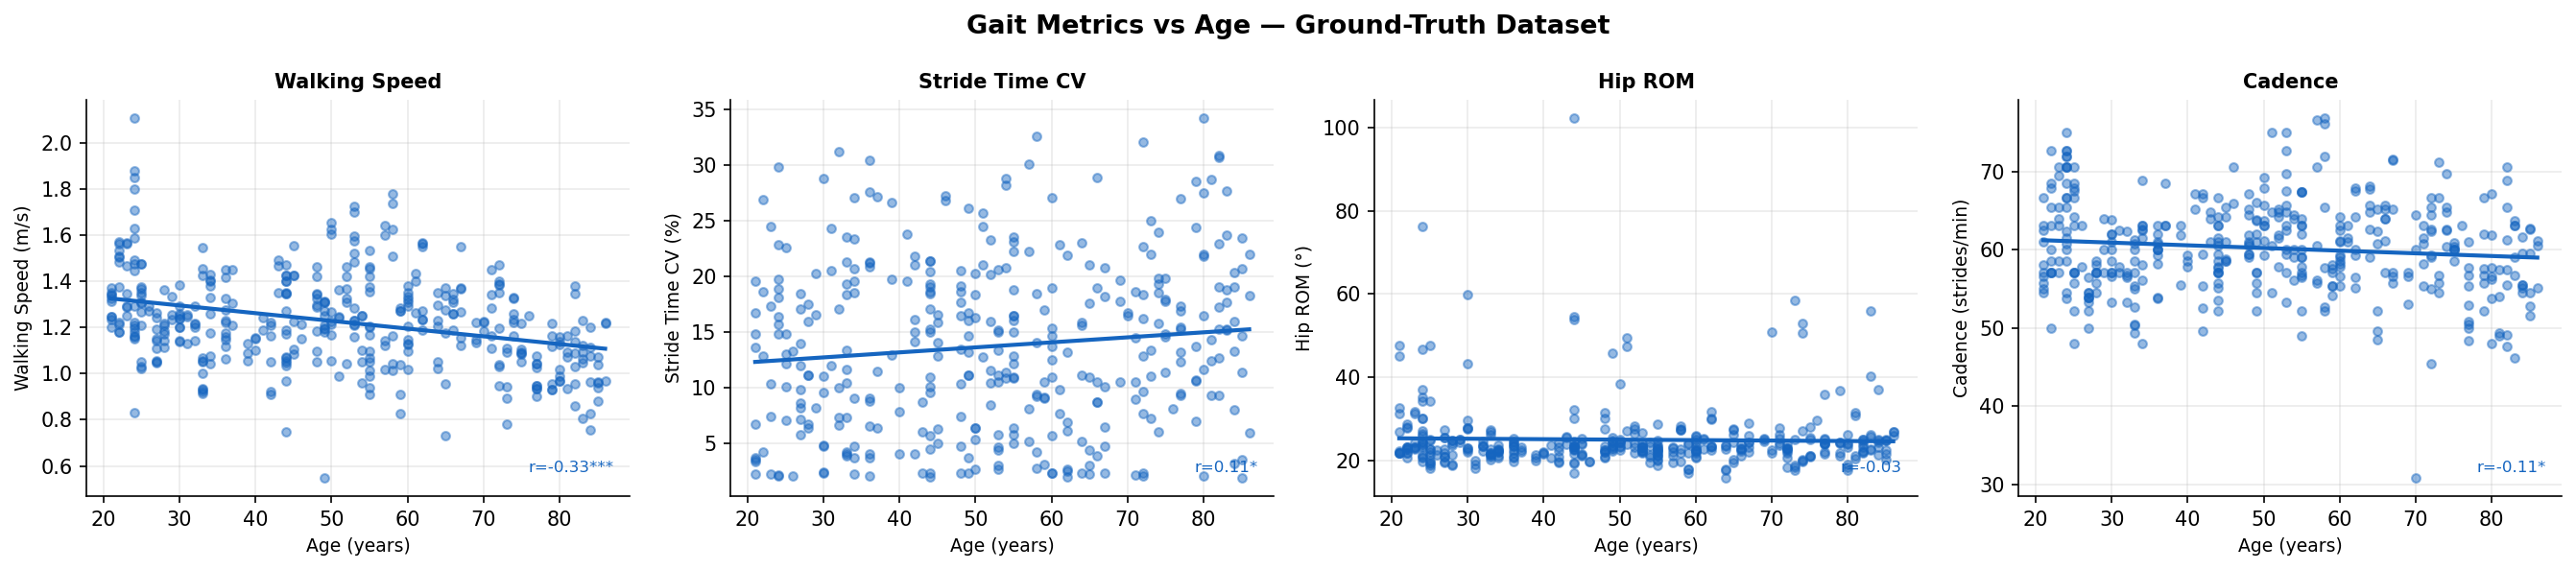
\includegraphics[width=\linewidth]{sec/figs/dataset/age_regression.png}}%
	{\fbox{\parbox[c][2cm][c]{\linewidth}{\centering Figure missing: \texttt{sec/figs/dataset/age\_regression.png}}}}
	\caption{Per-clip linear regression of clinical gait metrics against chronological age on the processed VC dataset.}
	\label{fig:age_regression}
\end{figure}

Per-clip regressions against chronological age (Fig.~\ref{fig:age_regression}) reproduce the expected directions across all four headline metrics, with weak-to-moderate negative correlations for walking speed, hip RoM, and cadence and a positive correlation for stride-time CV.

\subsubsection{Back-to-Back Evaluation of Generative Motion vs Dataset}
When evaluating the generated clips conditioned on age, the metrics reveal both the potential and the limitations of the LoRA-adapted model.
The generated motions successfully reproduce the expected age-related change in Range-of-Motion (RoM), with the \texttt{old} token producing significantly constrained hip RoM (21.5$^\circ$) compared to the \texttt{young} and \texttt{mid} tokens (24--25$^\circ$).
This indicates that the LoRA adapter successfully learns and imposes spatial kinematic constraints.

\begin{figure}[H]
	\centering
	\IfFileExists{sec/figs/combined/combined_violin.png}%
	{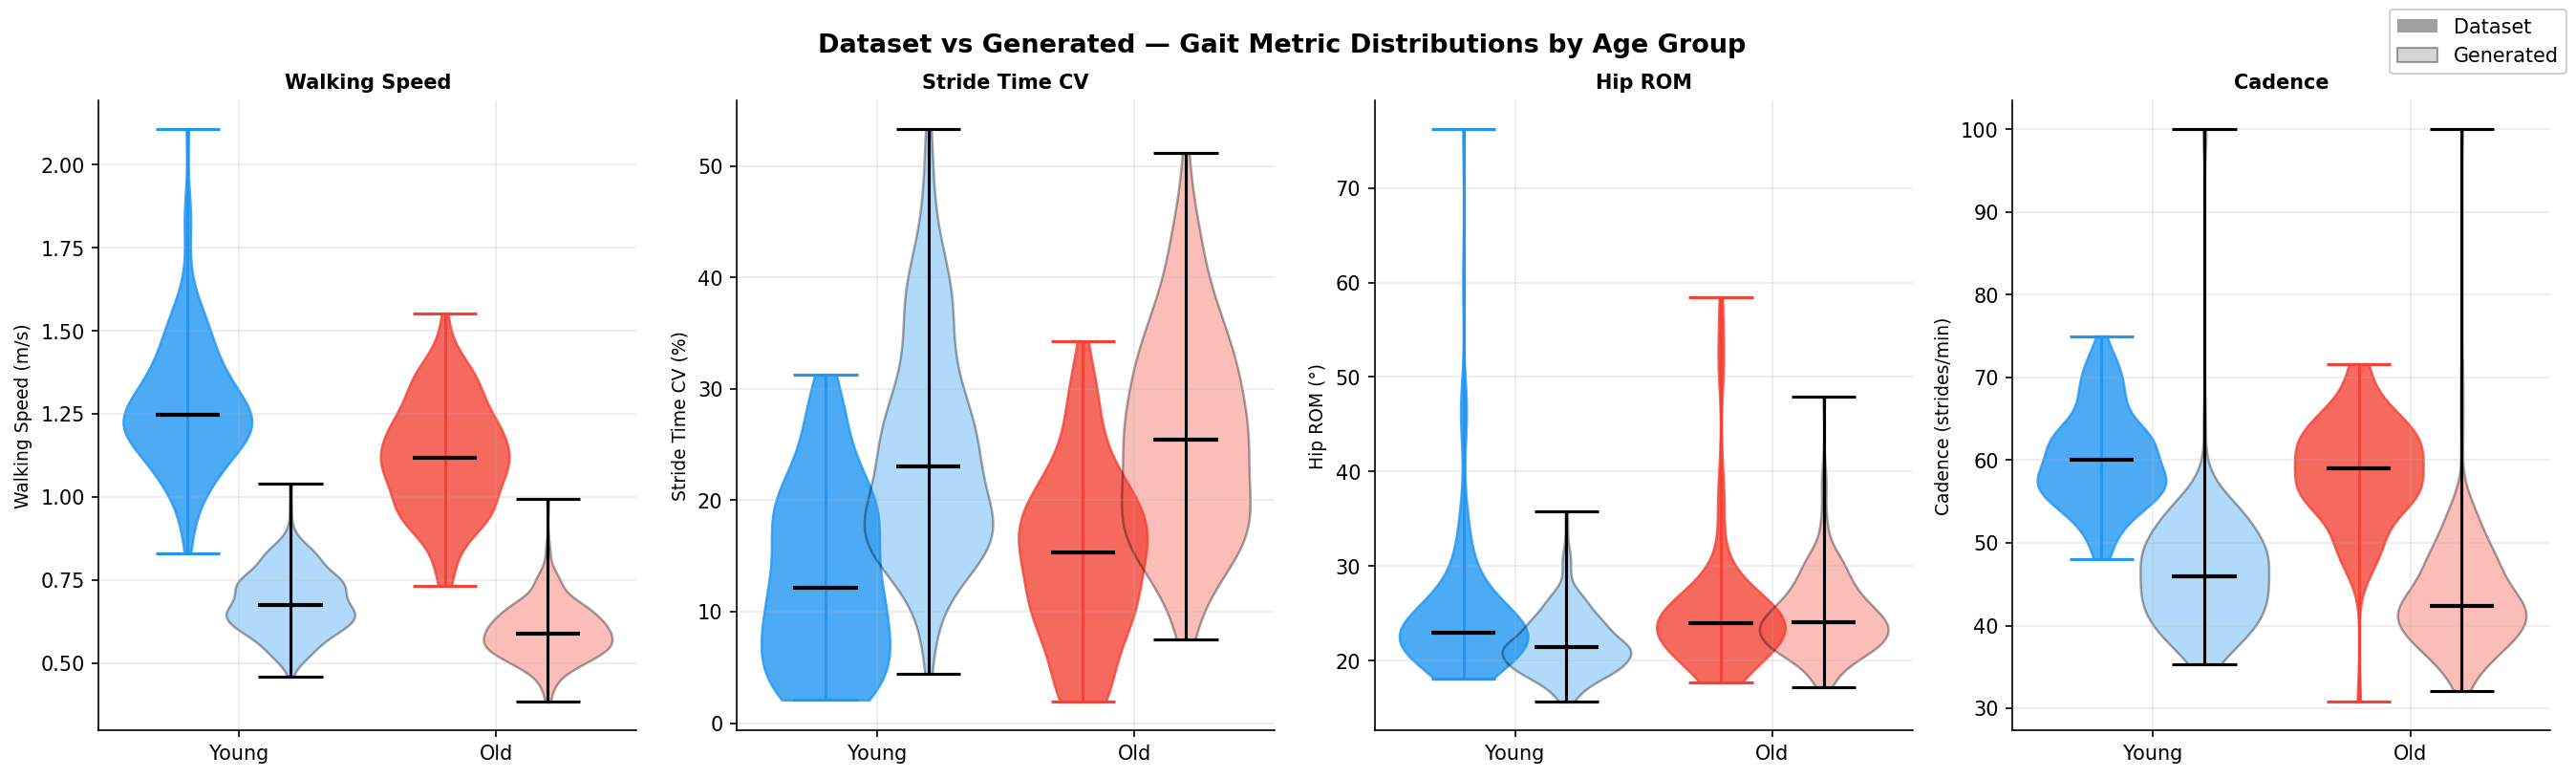
\includegraphics[width=\linewidth]{sec/figs/combined/combined_violin.png}}%
	{\fbox{\parbox[c][2cm][c]{\linewidth}{\centering Plot missing: \texttt{sec/figs/combined/combined\_violin.png}}}}
	\caption{Violin plots comparing the distribution of clinical metrics between the ground-truth dataset and the generated motion clips across age groups.}
	\label{fig:clinical_eval}
\end{figure}

Joint-speed profiles over the gait cycle (Fig.~\ref{fig:gait_cycle}) further confirm preserved age ordering: generated Young clips maintain higher peak joint speeds than generated Elderly clips, in agreement with the dataset trend.

\begin{figure}[H]
	\centering
	\IfFileExists{sec/figs/dataset/gait_cycle_speed.png}%
	{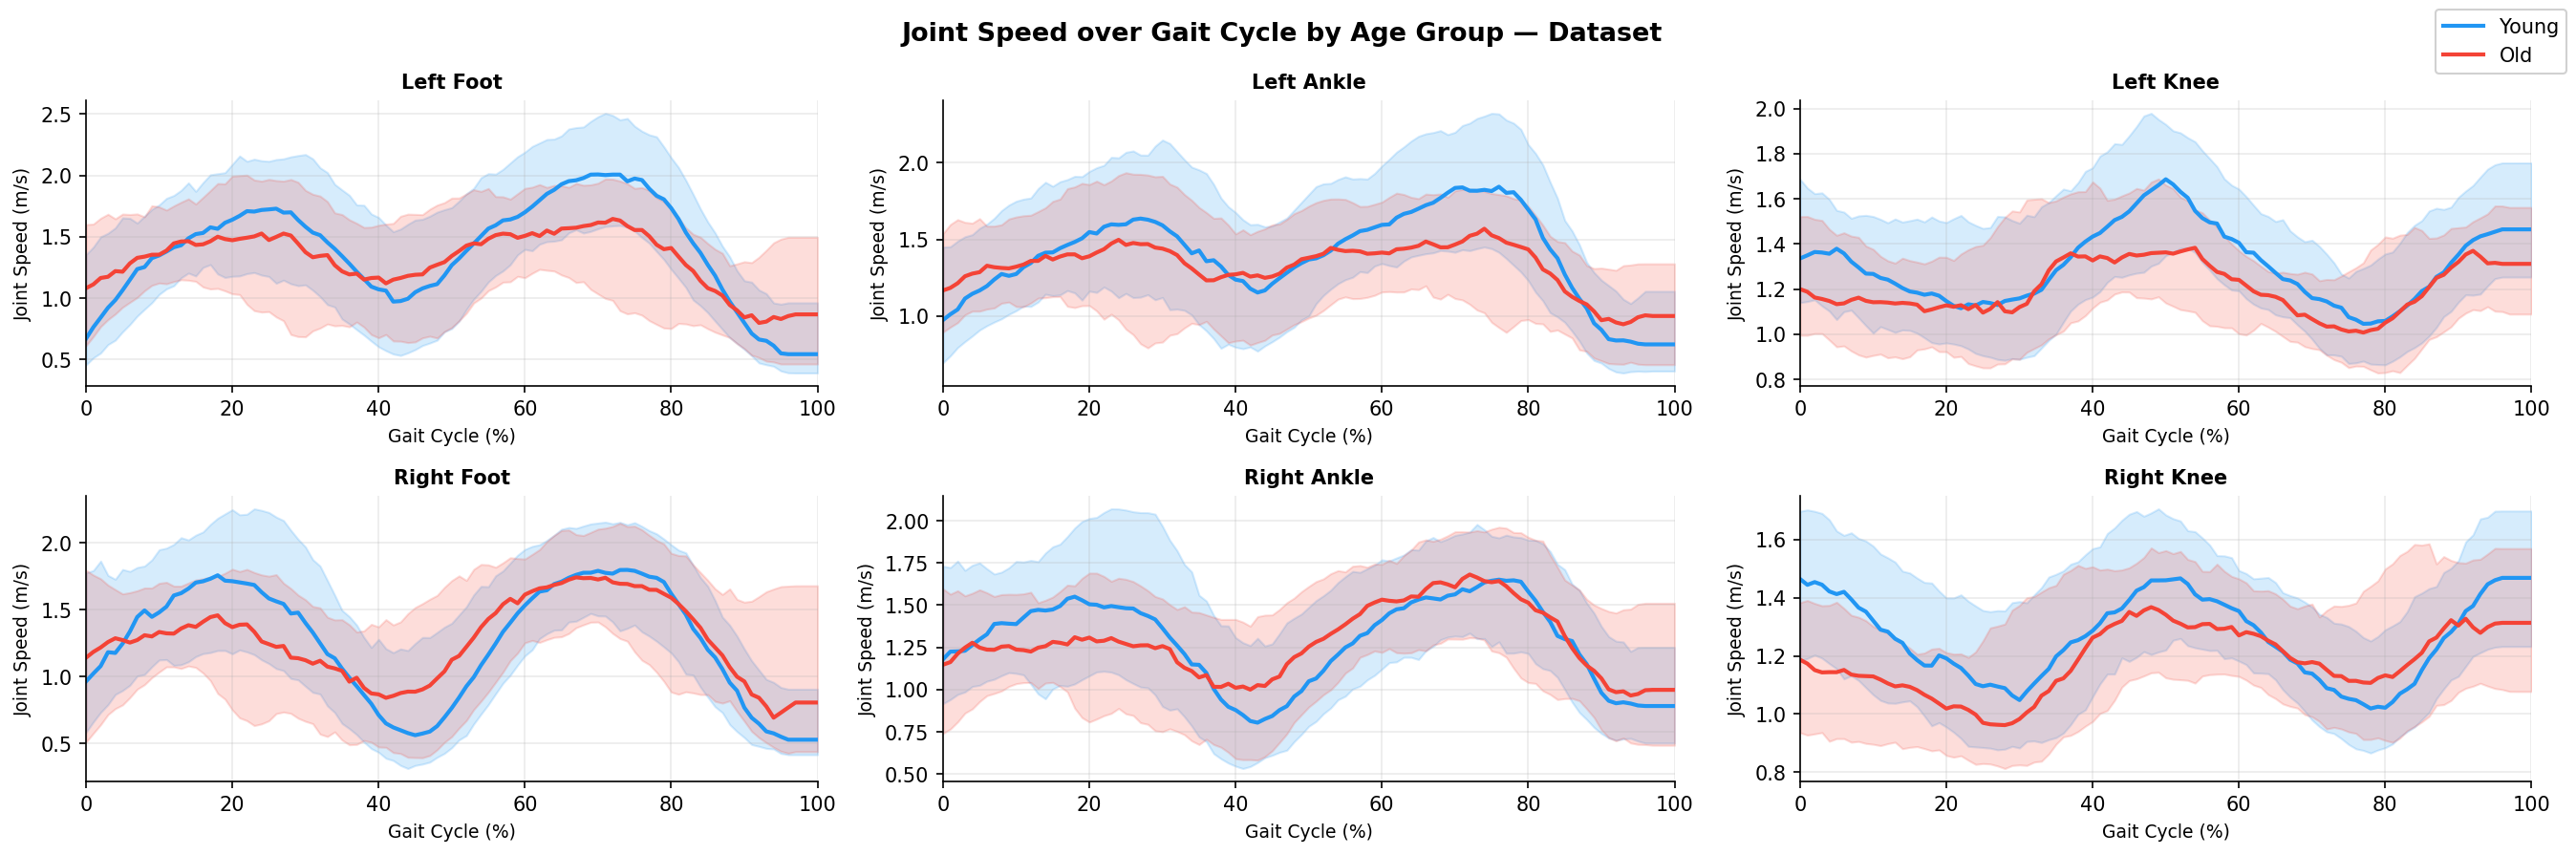
\includegraphics[width=\linewidth]{sec/figs/dataset/gait_cycle_speed.png}}%
	{\fbox{\parbox[c][1.5cm][c]{\linewidth}{\centering Plot missing: \texttt{sec/figs/dataset/gait\_cycle\_speed.png}}}}

	\vspace{0.3em}

	\IfFileExists{sec/figs/gen/gait_cycle_speed.png}%
	{
\includegraphics[width=\linewidth]{sec/figs/gen/gait_cycle_speed.png}}%
	{\fbox{\parbox[c][1.5cm][c]{\linewidth}{\centering Plot missing: \texttt{sec/figs/gen/gait\_cycle\_speed.png}}}}
	\caption{Joint speed over normalized gait cycle, averaged by age group. Top: ground-truth dataset. Bottom: generated motion clips.}
	\label{fig:gait_cycle}
\end{figure}

However, the generative model struggles with spatiotemporal consistency.
Critically, the stride Coefficient of Variation (CV) is uniformly elevated (16--19\%) across all generated clips, far exceeding clinical reference values.
We suspect that this might be due to the stochastic noise introduced in the diffusion process, which overwhelmed the stride consistency across samples.
